% !TEX root = ../../numb3rs.tex
\newpage
\subsection{302: Two Daughters\label{302}}

This is the sequel to Spree, Crystal tries to find her daughter and erase mistakes of her past. Crystal kidnaps Megan and the FBI team tries to capture her before someone else gets hurt. Charlie uses math to locate Crystal's position and understand what she is trying to accomplish. \\


%%%%%%%%%%
\temph{Changing the Rules of the Game}
%%%%%%%%%%

Charlie illustrated the fact that Tic-Tac-Toe is a game where there is no winner assuming that both players do not make mistakes. He point out that in order for a player to win one needs to change the rules a bit. Let us consider some variations of Tic-Tac-Toe. \\

\fbox{\begin{minipage}{43em}
\begin{center} \large \dotuline{Tangent}  \\ \end{center}
Tic-Tac-Toe is an ancient game, and it has been played since as early as 1300~BC by the Egyptians. It has many other names, and its simplicity makes it a good introductory example of a \bref{combinatorial game}{https://en.wikipedia.org/wiki/Combinatorial_game_theory}.
	\begin{figure}[H]
	   \centering
	   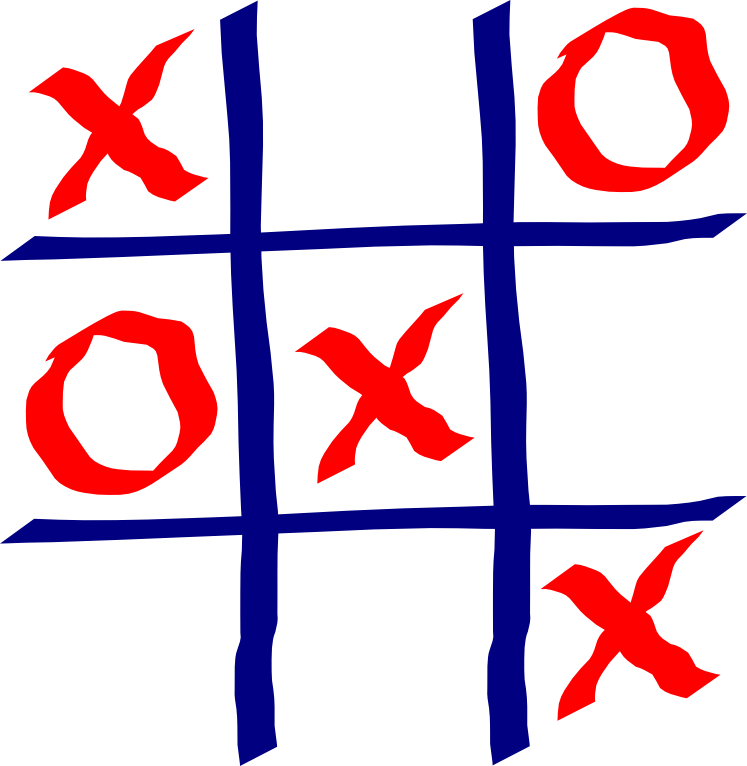
\includegraphics[width=0.25\textwidth]{season3/302/images/tictactoe.png} 
	\end{figure}
\end{minipage}} \vspace{0.2cm}


\fbox{\begin{minipage}{43em}
\begin{center} \large \dotuline{Activity 1}  \\ \end{center}
\begin{enumerate}[a.]
\item Suppose that the first player is allowed to make two moves consecutively. Show that the first player is always able to win.
\item Now suppose that both players are allowed to make two consecutive moves. Show that in this case the first player is also always able to win.
\item Suppose we now play Tic-Tac-Toe in a $3\times 3\times 3$ cube. Here a player wins if he/she is able to place three $X$'s (or 0's) in a row, column, or diagonal. This game can be won by either the first or second player (as supposed to a draw). Which player can always win? What is the winning strategy (list of moves) needed for that player to win?
\item Consider the following game: Two players take turns selecting integers from 1 to 9, without repetition. The player who is able to select three numbers (not necessarily in consecutive moves) so that their sum is 15 is the winner. Show that this game is just Tic-Tac-Toe in disguise.
\item Can you think of a version of Tic-Tac-Toe where the \emph{second} player is always able to win?
\end{enumerate}
\end{minipage}} \vspace{0.2cm}

%%%%%%%%%%
\temph{Trawler Boat Problem}
%%%%%%%%%%

When trying to rescue Megan, Charlie suggests using the solution to the Trawler Boat Problem to narrow down the possible locations of Crystal. The problem is the following: There are two boats traveling at constant speeds, and the faster boat is chasing the slower. At some point the slower boat enters a fog bank, and the faster boat cannot see it anymore. What should the faster boat do to catch the slower boat? In this episode, the FBI is the faster boat and Crystal is the slower boat. The solution is quite surprising, but before explaining it in detail, we simplify the problem a bit. Let us denote by $F$ the faster boat and by $S$ the slower boat, and let us say that $S$'s is moving at a speed of $v$~m/s. We also assume that the boats were moving in a straight line, and that the $S$ keeps moving in a straight line after $F$ cannot see it anymore (that is, $S$ just changed directions). \\

\fbox{\begin{minipage}{43em}
\begin{center} \large \dotuline{Tangent}  \\ \end{center}
The logarithmic spiral (a.k.a. equiangular spiral) was first described by \bref{Ren\'e Descartes}{https://en.wikipedia.org/wiki/Ren\%C3\%A9_Descartes} in 1638. Later \bref{Jakob Bernoulli}{https://en.wikipedia.org/wiki/Jacob_Bernoulli} named it spira mirabilis, latin for ``miraculous spiral'' because of the nice property that the size of the spiral increases but its shape is unaltered with each successive curve. Bernoulli was so fascinated by the curve that he asked that it be engraved on his head stone. Unfortunately the carver put an \bref{Archimedes spiral}{https://en.wikipedia.org/wiki/Archimedean_spiral} instead by accident. Perhaps people have described this curved as miraculous due to its presence in nature, as depicted below.
	\begin{figure}[H]
	  \centering
	  \begin{minipage}[b]{0.4\textwidth}
	    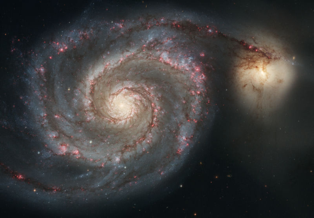
\includegraphics[width=\textwidth]{season3/302/images/galaxy.png}
	  \end{minipage}
	  \hspace{1cm}
	  \begin{minipage}[b]{0.37\textwidth}
	    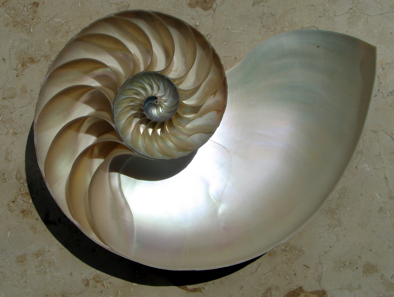
\includegraphics[width=\textwidth]{season3/302/images/shell.png}
	  \end{minipage}
	\end{figure}
\end{minipage}} \vspace{0.4cm} 



\noindent\textbf{\large Simplified Version} \\

Suppose that both boats start their movement at the same point $A$, and at the same time. The slower boat $S$ moves away from $A$, but the faster boat $F$ cannot see $S$'s direction, but knows that at time $t$ (in seconds), $B$ will be $vt$~meters away from $A$. So to catch $S$ it is enough for $F$ to be $vt$~meters away from $A$ at every moment. But since $F$ does not know $S$'s direction, it also needs to cover all possible directions $S$ might have chosen. To do this, $S$ needs to travel along a \bref{logarithmic spiral}{https://en.wikipedia.org/wiki/Logarithmic_spiral}. The picture below describes what is going on: The blue curve represents $F$'s movement, and the red line represents $S$'s movement. At time $t$, $S$ is at the intersection of the red line and the circle of center $A$ and radius $t$, while $F$ is at the intersection of the blue curve and the same circle. 
	\begin{figure}[H]
	   \centering
	   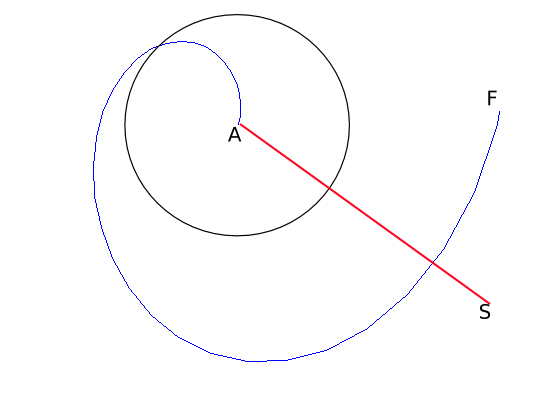
\includegraphics[width=0.4\textwidth]{season3/302/images/spiral.png} 
	\end{figure}
That is, at time $t$, $F$ is $vt$~meters away from $A$, just like $S$. So $F$ will eventually catch up with $S$, and this will happen at the intersection of both curves. \\

\noindent\textbf{\large Version in the Show} \\

Now let us revisit the original problem. Here the boats do not start at the same point, but the problem can be reduced to the simple version discussed above by taking island to be the point where the $S$ disappeared from $F$'s sight. \\

However, we do not need to go all the way to $A$ and the start the spiral. The solution is for $F$ to assume that $S$ is heading towards it. If this is the case, $F$ will catch it for sure, otherwise we move along the spiral with center the point where $S$ disappear. As before, $F$ and $S$ will both be at the same distance from $A$ (the point where $S$ disappeared) and $F$ will eventually catch $S$. A natural question to ask is \emph{how fast} does $F$ need to be traveling? You are given the chance of thinking about this exact question in Activity 2. \\

\noindent\textbf{\large Equations of the Logarithmic Spiral} \\

In polar coordinates, the equation for the logarithmic spiral is simply  $r=ae^{b\theta}$, where $a$ and $b$ are positive real numbers. Recall that in polar coordinates, $(r,\theta)$ represents the point at distance $r$ from the origin and angle $\theta$ from the horizontal line going through the origin. Doing the standard conversion $x(t) = r \cos t$ and $y(t) = r \sin t$ we get the parametric equations of this curve. It has the nice property that the angle $\phi$ between the tangent and radial line at the point $(r,\theta)$ constant. Since since $\frac{dr}{d\theta}=bae^{b\theta}=br$, the said property can be represented with the following equation below
	\[
	\phi=\arctan\left(\dfrac{r}{\frac{dr}{d\theta}}\right) = \arctan\left(\dfrac{1}{b}\right)
	\]

\fbox{\begin{minipage}{43em}
\begin{center} \large \dotuline{Activity 2}  \\ \end{center}
\begin{enumerate}[i.]
\item In the equations described for a logarithmic spiral, consider $\lim_{b\to 0} r$ and describe the curve obtained in this manner.
\item In the case as above, what is $\phi$ approaching?
\item Give conditions for $F$ to be able to catch $S$ in terms of $S$'s velocity. How fast must $F$ be traveling?
\end{enumerate}
\end{minipage}} \vspace{0.2cm}

%%%%%%%%%%
\temph{Galton Board}
%%%%%%%%%%

When the FBI team is closed to capture Crystal, Charlie (inadvertently) compares the situation to the Galton Board. The picture to the right describes the basic idea of this object. It consists of a funnel-shaped vertical board with nails arranged as the green dots in the picture, with transparent walls fixed by the nails. The Galton board is used to perform the following experiment: We place a ball at the top of the board (represented by the red dot) and let it fall until it falls in one of the containers at the bottom. If we repeat the experiment enough times, we will notice that the piles of balls describe a \bref{bell curve}{https://en.wikipedia.org/wiki/The_Bell_Curve}.The picture to the right has 5 rows of nails, but we can construct as many rows as we want.
	\begin{figure}[H]
	   \centering
	   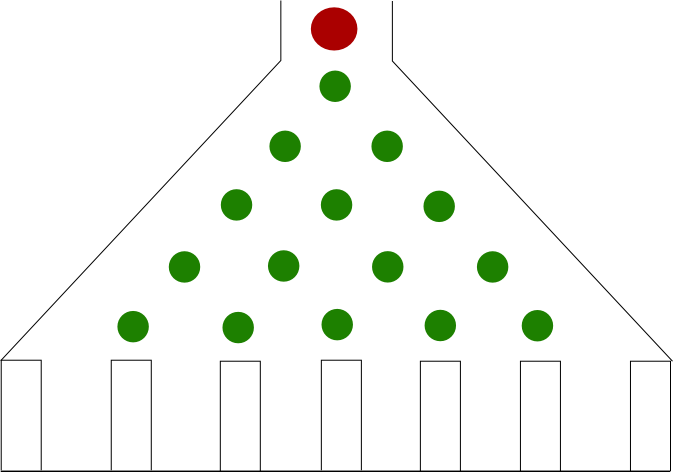
\includegraphics[width=0.25\textwidth]{season3/302/images/galton.png} 
	\end{figure}
Let us study what is going one in more detail. Notice that every time the ball hits a pin, it can either go to the right with some probability $p$, or go to the left with probability $q =1 - p$. One would expect that $p = q = \frac{1}{2}$, but the board could be built with a material that favors right turns. So it makes sense to make no assumptions about $p$ and $q$. Similarly, we assume that the board has $n$ rows of pins (with $n = 5$ in our picture). \\

To argue that the results of the experiment look like a bell curve, we notice that it is easier for a ball to fall in one of the containers in the middle of the board than at one of the containers at the extremes. This is because there are more ways to get to the center than, say, to the first container. For instance, the probability of a ball falling in the first container (from left to right) is $q^n$, since at each row we decided to go to the left each time. Now, let us compute the probability of a ball falling into the second container: Notice that in order for a ball to fall in the first container, it must have gone once to the right of a pin, and the rest of the time it must have gone left, and so there are $n$ paths that lead to the second container (why?). So the probability of falling into the second container is $npq^(n-1)$. In the activity below you are given the chance of computing the probabilities for a general board.


\fbox{\begin{minipage}{43em}
\begin{center} \large \dotuline{Activity 3}  \\ \end{center}
	\begin{figure}[H]
	   \centering
	   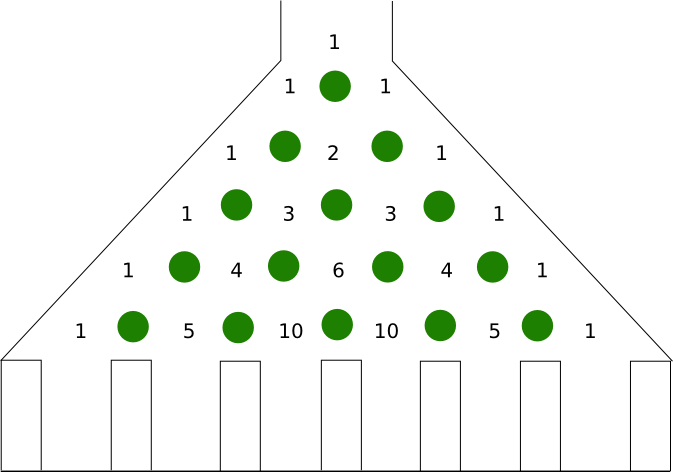
\includegraphics[width=0.4\textwidth]{season3/302/images/galton2.png} 
	\end{figure}
\begin{enumerate}[a.]
\item Recall the construction of \bref{Pascal's triangle}{https://en.wikipedia.org/wiki/Pascal's_triangle}. We can place the numbers of every row of Pascal's triangle between two nails and between the edge and the first and last row, as shown in the picture to the right. What are these numbers counting? It may be helpful to notice that the path a ball takes from the top to one of the containers can be encoded with a sequence of letters $L$ (for left) and $R$ (for right).
\item Using the picture to the right, and assuming that every time a ball hits a nail it has probability $p$ to go to the right and probability $q = 1 - p$ to go to the left, compute the probability of a ball to end up in the first container (from left to right). [Hint: If a ball ends up in the first container, then it must go to the left every time it hits a nail.] Do the same for all the other containers, and generalize the result for a board with $n$ rows. You will need the result from part (a.) to do this correctly.
\item Take $n = 6, p = q = \frac{1}{2}$. Use your results from (c.) to make a draw a graph in the $x$-$y$ plane, where $x = i$ represent the containers $i$ of the Galton board and $y$ being the probability of a ball reaching container $i$. Compare your points to a bell curve. This is an illustration that the \bref{normal distribution}{https://en.wikipedia.org/wiki/Normal_distribution} approaches the \bref{binomial distribution}{https://en.wikipedia.org/wiki/Binomial_distribution}.
\item Now suppose you want each ball to fall in the first 4 containers, so you place some obstacles on the board to avoid the balls from falling into the remaining containers. What is the minimal number of obstacles that you have to place?
\item In the situation of (d.), for each container, compute the probability of a ball ending up in it.
\end{enumerate}
\end{minipage}} \vspace{0.2cm}

